%\begin{savequote}[8cm]
%\textlatin{Neque porro quisquam est qui dolorem ipsum quia dolor sit amet, consectetur, adipisci velit...}

%There is no one who loves pain itself, who seeks after it and wants to have it, simply because it is pain...
%  \qauthor{--- Cicero's \textit{de Finibus Bonorum et Malorum}}
%\end{savequote}

\chapter{BLDA prioritizes accessible regulatory regions in MLL-AF4 driven leukemia} \label{ch4}

\minitoc



% remember to put the process of making the MLL specific blacklist on the 



% motifs
% n=5   
% topic 3 
    % NFYC diffexp in apl https://genomebiology.biomedcentral.com/articles/10.1186/gb-2008-9-2-r38
%   % AHR crucial for leukemia stem cell maintenance https://cancerres.aacrjournals.org/content/79/22/5799
%   % CUX1 involved in myeloid leukemias https://ashpublications.org/blood/article/121/6/975/31447/CUX1-is-a-haploinsufficient-tumor-suppressor-gene 
%   % ZFX https://pubmed.ncbi.nlm.nih.gov/24485662/
% 
% NEUROG2 is also enriched, the only one not associated with leukemia of some sort. 
% shown to create distinct chromatin accessibility landscapes in very distinct neuron subpopulations https://www.ncbi.nlm.nih.gov/pmc/articles/PMC6556771/

% topic 1
%   CREB1 is a "suspected leukemia ocoprotein" https://pubmed.ncbi.nlm.nih.gov/23000483/
%           also CREM found
%      bind cAMP response elements (cAMP-response element)
%       important for normal hematopoiesis https://www.ncbi.nlm.nih.gov/pmc/articles/PMC2214769/
%        Overly expressed both in the boen marrow and blast cells of acute leukemia patients
%   MAX is differentially expressed in human myloid leukemias https://pubmed.ncbi.nlm.nih.gov/7500645/

%  topic 2
%   LIN54 is a cell cycle gene which makes sense given its enrichement in normal pre b cells https://www.nature.com/articles/ncomms12301


% 30% of cells in the RS4;11 paper resembled myeloid cells cytochemically. 
%       they were from a relapsed patient https://pubmed.ncbi.nlm.nih.gov/3917311/#:~:text=A%20cell%20line%2C%20designated%20RS4,7.
%       morphologically, they were all lymphoid in appearance

% SEM cells also from a 5 year old in relapse 
%   Lymphoid cells but also had some myeloid antigens like CD13, CD15, and CD33 https://onlinelibrary.wiley.com/doi/pdf/10.1111/j.1365-2141.1994.tb04726.x?casa_token=wybBr2k2O-QAAAAA:M5peYc4iAuyTaA7HhoEKQd-IgOQ15B6dm9_EPi-Od1UZpl5aKSTUxYT2B8IXkgYkPlaq5QfJpmLDJqk


\section{Introduction} \label{ch5:intro}

\section{Methods} \label{ch5:methods}

\section{Results} \label{ch5:results}

\subsection{MLL-AF4 in the context of other blood cells}

\subsubsection{Identifying MLL-AF4 specific accessibility patterns}

Within the context of the entire ENCODE dataset, the MLL-AF4 cells were indistinguishable from the closely related B cell precursors. In order to identify any differences between them, the model would need a large number of topics, sufficient to explain all of the detailed similarities between the diverse set of celltypes represented in the dataset. Therefore, in this section I conduct a detailed examination of the MLL-AF4 cells and compare them to the B cell precursors with a smaller topic model. 

The number of called peaks differed significantly between experiments (\Cref{fig:mll_peak_calls}A). SEM and RS4;11 had the most peaks, while one of the patients had the lowest. In the latter case, it is suspected that the known low quality of this sample affected the sequencing, causing an anomalously low number of peaks to be identified. The remainder of the samples have an intermediate number of peaks, which will be taken into consideration when interpreting further analysis. 

\todo{Calculate the coverage of each sample and see whether SEM and RS4;11 here have higher coverage, leading to more peak calls. Tried this with megadepth but its giving very weird results (0.91X coverage for SEM? What?)}

In order to form \textit{a priori} expectations for the patterns to observe in the topic modelling approaches, we calculate the overlapped raw peaks for each of the different cell types (\Cref{fig:mll_peak_calls}B). Firstly, concentrating on the patient samples, we find that there are significant differences in peak sharing between other patients, B cell precursors, and MLL-AF4 cell lines (ANOVA P value = 0.0174). While they are no more similar to themselves than any other group (corrected $T$ test versus B cell precursors corrected P = 0.787, corrected $T$ test versus MLL-AF4 cell lines corrected P = 0.100), they do share significantly more peaks with the MLL-AF4 cell lines than they do with the B cell precursors (corrected $T$-test P value = 0.015). P values were corrected with Holm's method for multiple testing of three pairwise tests.

\subsubsection{An MLL-AF4 specific accessibility blacklist}

Cell lines maintained in culture accumulate genetic differences over time, some of which may be advantageous to their survival in culture. \cite{Liu2019}\textcite{Ben-David2018} studied the genetic baseline for the same cell line matured in different laboratories and identified copy number gains and loses, insertions and deletions (indels) and chromosomal translocations affecting large portions of the genome in cell lines which were not shared across laboratories. Latent structural differences between the cell lines in question and the reference genome pose a particularly concerning confounding factor to the interpretation of topic modelling; differences in mappability between regions reflected in abnormal peaks unrelated to biological differences between cell types would contaminate pathway and motif enrichment analyses. To ameliorate concerns associated with structural diversity in the RS4;11 and SEM cell lines within our laboratory environment, we construct a list of regions whose enrichment is solely due to technical issues such as biases in mappability.

To do so, we assemble collection of input tracks to ChIP-seq analysis conducted on the RS4;11 and SEM cells in question. Briefly, these input tracks represent sonicated DNA that has not been pulled down. As such, it represents a proxy for the genomic background of sequencing noise, and regions where pileups occur are theoretically devoid of any biological meaning, and therefore represent technical artifacts. Peak calling is performed using Macs2 with an extremely stringent Q value cutoff, 0.00001, in order to preserve as much of the accessible genome as possible while eliminating the most obvious signals of technical artifacts. The resulting merged blacklist contains 21068 short regions (average $\pm$ standard deviation length = 483 $\pm$ 342 base pairs) covering 10.1 megabases of sequence in total. This blacklist is combined with the blacklist of accessible regions from the ENCODE project (CITE). The combined list covers 21.3 megabases of sequence, which we exclude from all subsequent analyses.

\begin{figure}
    \centering
    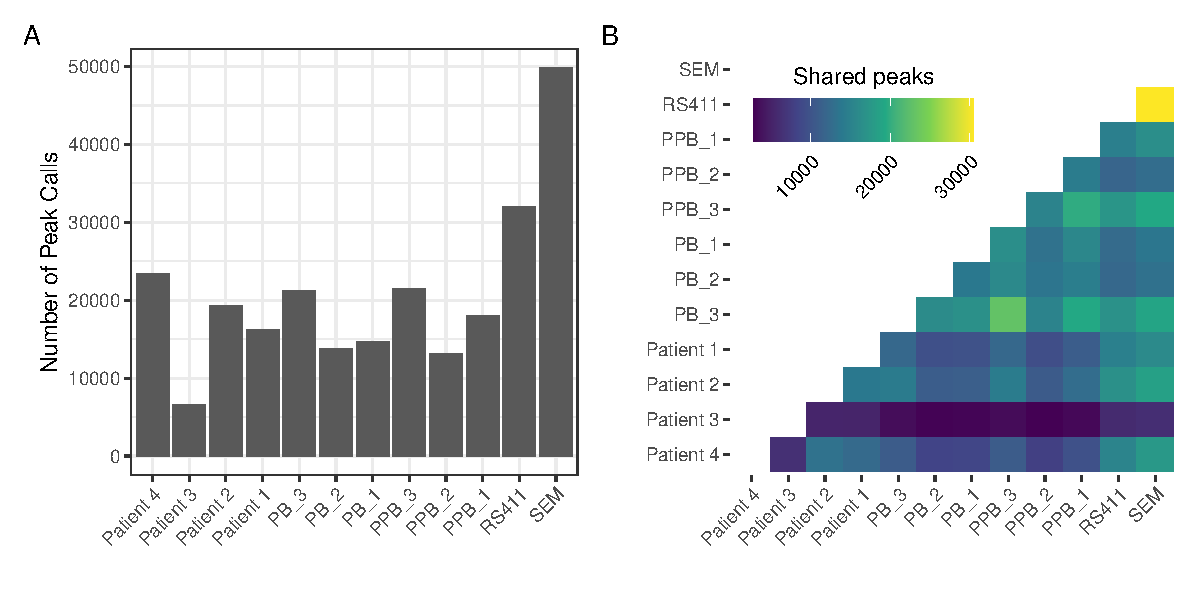
\includegraphics[width=\textwidth]{plot/ch5/mll_shared_peaks.pdf}
    \caption{Peak calling of MLL-AF4 and B Cell Precursor cells with LanceOTron. A. Raw number of peak calls per cell. B. Number of shared peak calls between pairs of cells.}
    \label{fig:mll_peak_calls}
\end{figure}

\subsubsection{Differential Accessibility between B cell Precursors and MLL-AF4 cells} \label{ch5:mll_diffacc}

\todo{EdgeR for diffAcc between all patients / RS411 and PPB}

\subsection{Topic modelling for MLL-AF4 cells}

Building on the baseline expectations obtained from the EdgeR differential accessibility analysis in \Cref{ch5:mll_diffacc}, we begin our investigation into the use of topic modelling to discover novel pathways that differentiate MLL-AF4 cells and normal B cell precursors. Peak calling is performed with LanceOTron and a score threshold of 0.5, as recommended. We construct a count matrix using the normalized read counts under each peak with BLDA as well as a one-hot encoded matrix for comparison.  Hyper-parameters alpha and beta are set for a given number of topics $k$ using Bayesian optimization and loadings are inferred using cisTopic and BLDA. 

We infer topic loadings for $k=5,\ldots,12$ topics (\Cref{fig:mll_all_topic}). The upper end of this range was chosen as the number of cells in the analysis. Visually, BLDA produces more specific topic loadings than does the one-hot encoding method, though the OHE is able to differentiate between the different classes, unlike in previous analyses.  Remarkably, very little substructure is detected within the B cell precursor population. When topics are inferred to be active in the B cell progenitors, they tend to be active in all of them (\Cref{fig:mll_shared_topics}). The MLL-AF4 patients show a complex relationship to the B cell precursors and cell lines, indicative that their regulatory programs are highly heterogenous. Patients 1 and 2 occasionally share topic loadings with the pan-\gls{bcp} grouping, with Patient 2 sharing much more frequently than Patient 1. Patients 3 and 4 however tend to be sufficiently heterogeneous to be split into seperate topics, and rarely are co-encriched with either the MLL-AF4 cell lines or the \glspl{bcp}. Both cell lines show some similarity to the \glspl{bcp}, with SEM sharing topic loadings more frequently than RS4;11 for any threshold. Interestingly, SEM is co-enriched for topics with the \glspl{bcp} more frequently than with RS4;11. Additionally, topics are very infrequently co-enriched at the level of 0.25 or above, meaning one quarter of the cell type's total topic contributions. This indicates that topics either tend to be hyper-specific, as is the case for RS4;11 in the $k=5$ case, or weakly shared between many cell types, as is the case for for the patients and \glspl{bcp} in the $k=10$ cases.

\begin{figure}
    \centering
    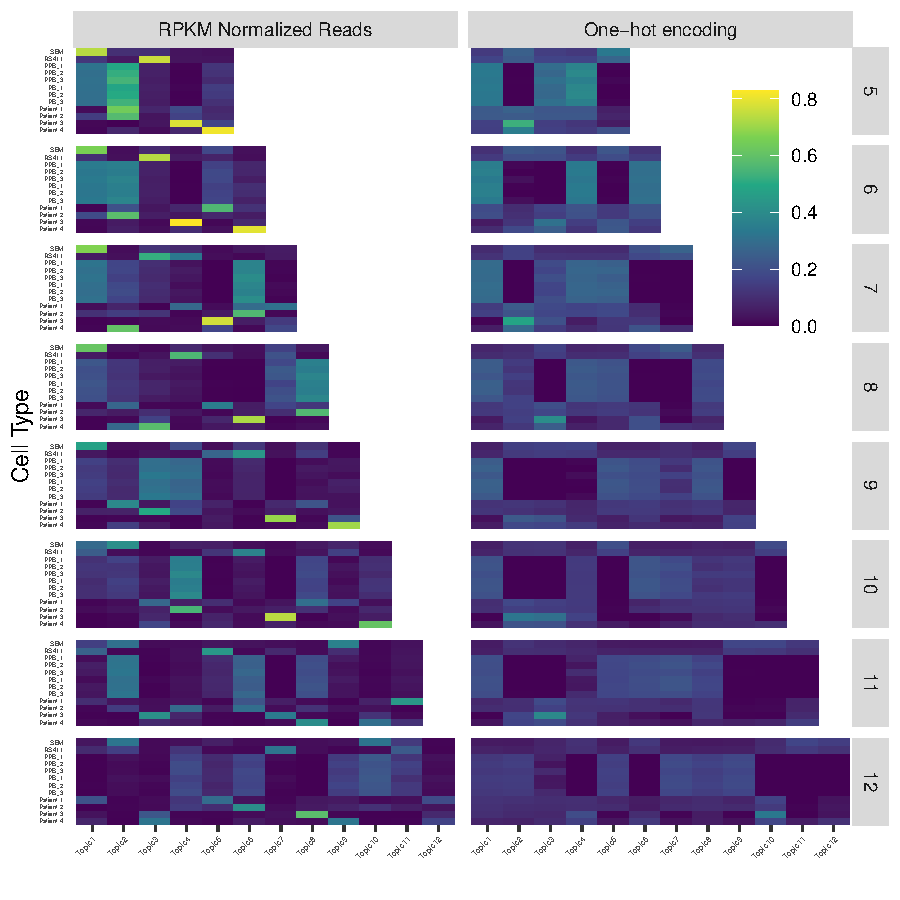
\includegraphics[width=\textwidth]{plot/ch5/mll_all_topics.pdf}
    \caption{Inferred topic loadings for $k = 5, \ldots, 12$ topics comparing MLL-AF4 cells to B cell precursors. RPKM normalised refers to the count matrix used to infer the topic loadings by BLDA, while one-hot encoding simply annotates which regions are called as peaks by LanceOTron. Topic loadings are normalised such that the sum of all topics within a cell equals one.}
    \label{fig:mll_all_topic}
\end{figure}

\begin{figure}
    \centering
    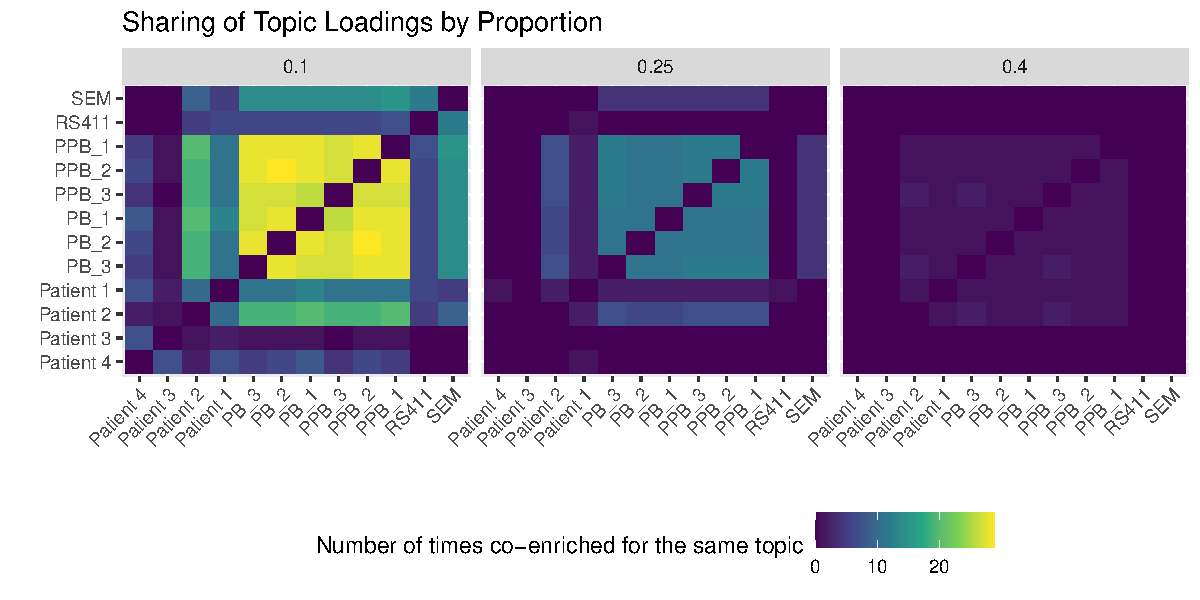
\includegraphics[width=\textwidth]{plot/ch5/mll_coenriched.pdf}
    \caption{Degree of shared topic activity between cell types. Plotted are the number of instances where a topic is active at the facetted level in both of the indicated cell types. Results are tabulated across all $k=5, \ldots, 12$ inference runs.}
    \label{fig:mll_shared_topics}
\end{figure}

Due to the high degree of topic coenrichment within the \glspl{bcp}, inference with the higher values of $k$ tends to spuriously split topic loadings. This is evident in both the OHE and BLDA cases, where the average topic loadings are very low for higher values of $k$. Additonally, RS4;11 is almost always annotated as having at least highly specific topic loading (topic 3 in $k=5, 6$, topic 4 in $k=8$). The utility of forcing a high number of topics on this system is, therefore, questionable.

For these reasons, we initially focus our examination on the smallest number of topics (\Cref{mll_k_5}). Many of the previously mentioned trends are even more evident in this small system.

\begin{figure}
    \centering
    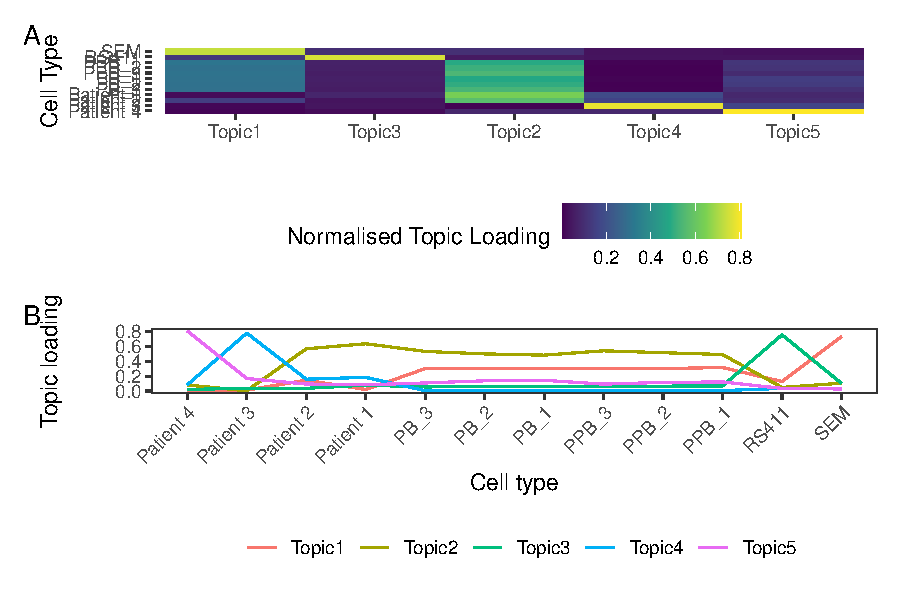
\includegraphics[width=\textwidth]{plot/ch5/mll_k_5.pdf}
    \caption{Inference for $k=5$ BLDA topic model. A. Normalized topic loadings by cell type. B. Normalized topic loadings displayed over cell types coloured by topic. }
    \label{fig:mll_k_5}
\end{figure}